\begin{figure}[h!]
	\centering
	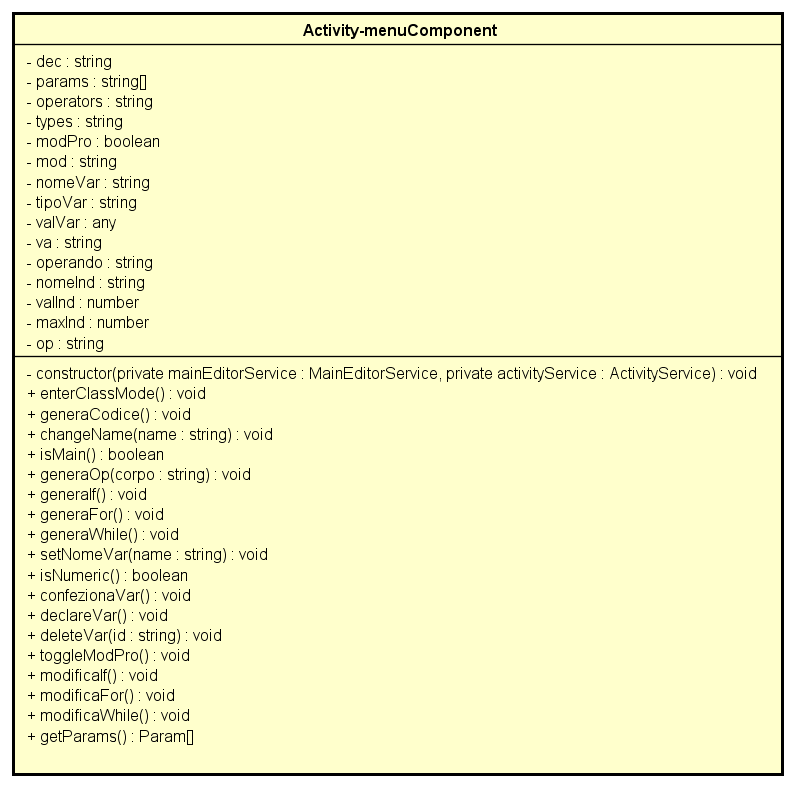
\includegraphics[scale=0.8]{res/sections/SpecificaFrontEnd/Components/Disegnetti/activity-menu.png}
	\caption{Diagramma della classe Activity-menu}
\end{figure}

\begin{itemize}
	
	\item \textbf{Descrizione:}\\
	
	\item \textbf{Utilizzo:}\\
	
	\item \textbf{Attributi:}
		\begin{itemize}
			\item \emph{-decisions: string[]}\\
			
			\item \emph{-dec: string}\\
			
			\item \emph{-params: string[]}\\
			
			\item \emph{-operators: string}\\
			
			\item \emph{-types: string}\\
			
			\item \emph{-modPro: boolean}\\
			
			\item \emph{-mod: string}\\
			
			\item \emph{-nomeVar: string}\\
			
			\item \emph{-tipoVar: string}\\
			
			\item \emph{-valVar: any}\\
			
			\item \emph{-va: string}\\
			
			\item \emph{-operando: string}\\
			
			\item \emph{-nomeInd: string}\\
			
			\item \emph{-valInd: number}\\
			
			\item \emph{-maxInd: number}\\
			
			\item \emph{-op: string}\\
			
		\end{itemize}
	\item \textbf{Metodi:}
		\begin{itemize}
			\item \emph{-constructor(private mainEditorService: MainEditorService,
		private activityService: ActivityService)}\\
    		\\
    		\textbf{Parametri:}
    		\begin{itemize}
    			\item \emph{mainEditorService: MainEditorService}\\
    			
    			\item \emph{activityService: ActivityService}\\
    			
    		\end{itemize}
    		\item \emph{+enterClassMode()}\\
    		
    		\item \emph{+generaCodice()}\\
    		
    		\item \emph{+changeName(name: string)}\\
    		\\
    		\textbf{Parametri:}
    		\begin{itemize}
    			\item \emph{name: string}\\
    			
    		\end{itemize}
    		\item \emph{+isMain()}\\
    		
    		\item \emph{+generaOp(corpo: string)}\\
    		\\
    		\textbf{Parametri:}
    		\begin{itemize}
    			\item \emph{corpo: string}\\
    			
    		\end{itemize}
    		\item \emph{+generaIf()}\\
    		
    		\item \emph{+generaFor()}\\
    		
    		\item \emph{+generaWhile()}\\
    		
    		\item \emph{+setNomeVar(name: string)}\\
    		\\
    		\textbf{Parametri:}
    		\begin{itemize}
    			\item \emph{name: string}\\
    			
    		\end{itemize}
    		\item \emph{+isNumeric()}\\
    		
    		\item \emph{+confezionaVar()}\\
    		
    		\item \emph{+declareVar()}\\
    		
    		\item \emph{+deleteVar(id: string)}\\
    		\\
    		\textbf{Parametri:}
    		\begin{itemize}
    			\item \emph{id: string}\\
    			
    		\end{itemize}
    		\item \emph{+toggleModPro()}\\
    		
    		\item \emph{+modificaIf()}\\
    		
    		\item \emph{+modificaFor()}\\
    		
    		\item \emph{+modificaWhile()}\\
    		
    		\item \emph{+getParams()}\\
    		
		\end{itemize}
\end{itemize}